
\documentclass{sig-alternate}
\conferenceinfo{GECCO}{'15, Madrid, Spain}
\usepackage{graphicx}
\usepackage{subfigure}
\usepackage{multirow}
\graphicspath{{pics/}}
\usepackage{listings}
\usepackage{amsmath}
\usepackage[sort]{natbib}
%\usepackage[]{algorithm2e}


\begin{document}

\title{Deep Parameter Optimisation}

\numberofauthors{2} %  in this sample file, there are a *total*
% of EIGHT authors. SIX appear on the 'first-page' (for formatting
% reasons) and the remaining two appear in the \additionalauthors section.
%
\author{
% You can go ahead and credit any number of authors here,
% e.g. one 'row of three' or two rows (consisting of one row of three
% and a second row of one, two or three).
%
% The command \alignauthor (no curly braces needed) should
% precede each author name, affiliation/snail-mail address and
% e-mail address. Additionally, tag each line of
% affiliation/address with \affaddr, and tag the
% e-mail address with \email.
%
% 1st. author
\alignauthor Fan Wu, Mark Harman, Yue Jia and Jens Krinke\\
       \affaddr{CREST, UCL, London, UK}
       %\affaddr{London, UK}
       %\affaddr{London WC1E 6BT, United Kingdom}\\
       %\email{fan.wu.12@ucl.ac.uk}
% 2nd. author
\alignauthor Westley Weimer\\
       \affaddr{University of Virginia}\\
       \affaddr{USA}
}
% There's nothing stopping you putting the seventh, eighth, etc.
% author on the opening page (as the 'third row') but we ask,
% for aesthetic reasons that you place these 'additional authors'
% in the \additional authors block, viz.
% Just remember to make sure that the TOTAL number of authors
% is the number that will appear on the first page PLUS the
% number that will appear in the \additionalauthors section.

\maketitle
\begin{abstract}

%
%An efficient memory allocator can help operating system save memory and make program applications run faster. This paper introduces a deep parameter optimisation technique to improve two non-functional properties, memory consumption and execution time for general purpose memory allocators. The approach extracts deep and shallow parameters to  adaptively re-tuning a memory allocator for a given specific program.
%We report experiments that show the deep parameter optimisation competes with the shallow parameter optimisation and the default configurations. For \# real world subjects, the deep parameter optimisation saves x\% of memory and reduce y\% of execution time overall.  We also present reasons why the implicit parameters exposed by our approach are meaningful to human developer. Deep parameter optimisation is thus a promising way to improve non-functional property for memory allocators.
%

\end{abstract}

% A category with the (minimum) three required fields
\category{H.4}{Information Systems Applications}{Miscellaneous}
%A category including the fourth, optional field follows...
\category{D.2.8}{Software Engineering}{Metrics}[complexity measures, performance measures]

\terms{Theory}

\keywords{Parameter tuning, parameter exposure, dynamic memory allocator} % NOT required for Proceedings



\section{Introduction}

To achieve optimal performance, many software systems need to be configured according to various workload and running environment. 
Software developers often expose a set of parameters for users to re-configure such software systems adaptively.
However, manual parameter tuning is a demanding challenge. Because users are required to not only have extensive knowledge about the system and the workload but also to balance many competing objectives, such as memory consumption and execution time.

Many work has risen to the challenge of automated parameter tuning\cite{Hoffmann:2011:DKR:1961296.1950390}. Early work attempted to find optimal values with mathmatical approaches \cite{Vuduc01statisticalmodels,autotuning,Whaley:1998:ATL:509058.509096,Tapus:2002:AHT:762761.762771} while SBSE\cite{Harman:2007:CSF:1253532.1254729} has been used in more recent research \cite{hutter2009paramils,arcuri-ssbse-2011,Hoffmann:2011:DKR:1961296.1950390}. Although these approaches can automatically re-configure a system under optimisation, they only provide limited improvements because they can only turn the parameters specified by system designer.

Many software systems contain undocumented internal variables and expressions which could also affect the performance of the software. However, identifying these variables and expressions is very difficult for general users, as it requires a deep understanding of the source code of the system. 

In this paper, we propose an automatic technique to discover the internal variables and expressions which cannot be accessed from changing the exposed parameters, but have greatly impacts on non-functional properties of interests. Our goal is to expose new parameters which can be used to change the values for these hidden variables and expressions. To distinguish with parameters exposed by software designer (Shallow Parameters), we name these new parameters Deep Parameters. As changing shallow parameters cannot directly change the internal code elements represented by deep parameters, the deep parameters thus provide additional opportunities in automated parameter tuning.

There has been an attempt to automate the process of exposing deep parameters with Software Tuning Panel for Autonomic Control (STAC)\cite{Brake:2008:ADS:1370018.1370031}. STAC first generates a design graph for a subject under optimisation. The design graph represents data reference transition flows in the subject. It then converts shallow parameters into sub-graph patterns. To discover deep parameters, STAC searches for similar sub-graph patterns in the complete design graph. 

Although STAC can discover some deep parameters effectively, it surfers from two limitations. First, STAC requires initial human effort to characterise shallow parameters. Second, STAC can only find a subset of deep parameters which have similar data transition patterns as the known shallow parameters. To overcome these limitations, we apply a mutation based sensitivity analysis to fully automated the process of locating the potential deep parameters and applies NSGAII to search for  optimal values to balance non-functional properties of interests. 

We illustrate the approach by reconfiguring a general purpose memory allocator,\emph{Dlmalloc}. We choose this application as an example, because many research has attempted to turn \emph{Dlmalloc} \cite{Risco-Martin:2009:ODM:1569901.1570116,RiscoMartin2010572}. In this paper, we focused on two non-functional properties, memory consumption and execution time, which are essential objectives to memory allocator. We evaluate our approach using four applications including benchmarks for \emph{Dlmalloc} and real world applications.

The paper presents evidence to suggest that the deep parameter optimisation is an effective approach to improve non-function properties for \emph{dlmalloc}. 
We report experiments that show the deep parameter optimisation competes with the shallow parameter optimisation and the default configurations. For all of our subjects, the deep parameter optimisation saves x\% of memory and reduces y\% of execution time overall. Moreover we also present reasons why the implicit parameters exposed by our approach are meaningful to human developer. The contributions of the paper be summarised as follow.


\begin{enumerate}

\item We introduce a automated approach to discover deep paramerts. 

\item We report the results of an empirical study comparing the shallow parameter tuning approach with our approach. On \# real world applications, the results show that our approach can save x\% of memory and reduce y\% of execution time over shallow parameter tuning. 

\item We also report a further case study on the implicity parameters found by the mutation based sensitivity analysis. The results suggest that these parameter are meaningfull to human developer and are good candidates to be promoted into explicit parameters. 

\end{enumerate}

%The rest of this paper is organised as follows. 
%Section 2 introduces the background of memory management and a popular general-purpose memory allocator \emph{dlmalloc}.
%Section 3 describes out adaptive deep parameter tuning approach.
%Section 4 explains the experimental methods for the empirical study, the results of which are discussed in Section 5
%Section 6 discusses related work, and the paper concludes with Section 7.




\section{Motivating Example}

We illustrate the idea of deep parameters with an example found by our approach for \emph{dlmalloc}.

\begin{figure}[ht]
\begin{lstlisting}
1 static void* sys_alloc(mstate m,size_t nb) 
2 {
3 ...
4 if (ss == 0) //check if first time through
5 { 
6     char* base = (char*)CALL_MORECORE(0);
7 ...
8 }
\end{lstlisting}
\vspace{-1.5em}
\caption{\emph{sys\_alloc} function in \emph{dlmalloc}}
\label{exp}
\end{figure}

Figure \ref{exp} shows a part of the \emph{sys\_alloc} function in \emph{dlmalloc}. We explain its internal operation here to illustrate to the reader that this clearly is a non-trivial optimisation problem. Of course, our parameter exposing and search-based tuning are general purpose techniques that have no knowledge of how \emph{dlmalloc} operates. To efficiently manage memory, \emph{dlmalloc} maintains an internal structure to organize the heap for memory reuse. Only when \emph{dlmalloc} cannot find a suitable chunk of memory for a memory request, does it call \emph{sys\_alloc()} to extend the current heap.

After applying the mutation analysis, we found mutants generated from mutating Line 6 have a notable affect on the memory consumption and the execution time of \emph{dlmalloc}. We take a close took at Line 6. It calls the \emph{CALL\_MORECORE}() function, which takes an integer as input. $CALL\_MORECORE()$ is a system call which extends or shrinks the current heap and returns the new address of the heap. $CALL\_MORECORE(0)$ neither extends nor shrinks the heap but simple returns the current address of heap, which is the original purpose of Line 6 mentioned above.
%In line 4, the $ss == 0$ return true if $sys_alloc$ is the first time being invoked, so line 6 can only be executed once at the beginning.

Thus changing the input value for $CALL\_MORECORE()$ in Line 6 allows us to control the amount of pre-allocated memory. However, although \emph{dlmalloc} provides several tuneable parameters to programmers, allowing them to adjust behaviors (see Section 5 for details), none of these shallow parameters can affect the $CALL\_MORECORE()$ function directly. To exposed a deep parameter $D$, our tool would transform Line 6 into the code below, where $D$ is the deep parameter exposed for users to control the pre-allocated heap.

\begin{lstlisting}
char * base = (char*)CALL_MORECORE(0 + D);
\end{lstlisting}

The proper size of pre-allocated memory depends on the specific program using this memory allocator. If the pre-allocated memory is too large, it could be a waste of memory. On the other hand, if it's too small, soon \emph{dlmalloc} will call $CALL\_MORECORE()$ again to extend the heap, thus wasting time. By tuning the deep parameter $D$, users can balance the time and space consumption. This is one example of a potential deep parameter. In our mutation analysis experiments, our tool ``discovers'' that changing the value of this deep parameter, it can reduce \#\% to \#\% of memory consumption in two of our subjects.


\section{Deep Parameter Optimisation}
\label{sec_deep_parameter_optimisation}

Figure~\ref{system} shows the work flow of our deep parameter optimisation. The approach takes the source code of the program, a set of test data and a set of non-functional properties of interest. 
It first applies mutation analysis and a non-dominated rank algorithm to discover potential locations for deep parameters, as explained in Section~\ref{discovering}. It then exposes deep parameters based on the type of expressions found at the locations (Section~\ref{exposing}). Finally, to tune the program, a multi-objective search-based algorithm is used to search for optimised values for both shallow and deep parameters (Section~\ref{sec_nsgaii}).

\begin{figure}[htbp]
\centering
\scalebox{0.55}{\includegraphics[width=6.2in]{pics/new_system}}
\vspace{-2em}
\caption{Deep parameter optimisation workflow. Given a program, test suite and non-functional properties, our approach applies mutation analysis, exposes deep parameters, and optimise them.}\label{system}
\end{figure}

\subsection{Discovering locations for deep parameters}
\label{discovering}
The first step is to identify potential locations at which we could expose deep parameters. 
In our approach, we represent the input program as an abstract syntax tree and a potential location $L$ is an expression node of the AST. 
We want to find a set of locations $L_D$ such that when we tune the value of the expression at $L_D$, some non-functional properties of the program could be improved while the program retains identical functional behaviour.
%We use software testing to valid the functional behaviour of the program. 
%To valid the functional behaviour of the tuned program, we test the tuned program with the input test set and compare the output with the test output of the original program.
We use a suite of regression test data to validate the correctness from the optimisation, following other established Genetic Improvement approaches~\cite{justyna2013, Langdon:2014:IMI:2576768.2598244}. We assume the presence of a test suite with each target application.

We use mutation analysis to automate the process of searching for locations
$L_D$. Mutation analysis deliberately makes simple syntactic changes to the
input program, to create a set of various versions of a program called mutants,
each containing a different syntactic change~\cite{5487526}. A
transformation rule that generates a mutant from the input program is known
as a mutation operator. By carefully choosing mutation operators, we can
use mutants to simulate the effect of making changes at those locations $L$s
from which a potential deep parameter may be exposed. 
% FIXME: Wes does not understand what "simulate the effects of making
% changes at _all_ protential locations" means in the previous sentence.
% Please clarify for the reader. 
% Fan tried to say that, using Mutation Operators, we can simulate
% changes to those locations from which a deep parameter may be exposed,
% thus to aid selecting most sensitive locations.
Table~\ref{tab:cmop} lists the operators we used to generate
mutants, covering locations of constants, relational, logical and
arithmetic expressions. 
% FIXME: Walk us through two operators chosen from tab:comp. Why are they
% good? Why did you pick them? Are they just like MOTHRA? This is a
% contribution of your paper. Elaborate!
% Yue added the following sentence.
These so-called `selective' mutation operators
have been widely used in mutation analysis experiments~\cite{5487526}.

\iffalse
\begin{table*} [ht]
\caption{Selected mutation operators}
\label{tab:cmop} 
\begin{center}
\begin{tabular}{ | c | l | l |}
  \hline
  Mutation Operators & Brief Description & Details \\ 
\hline
  CRCR & Required constant replacement & Replace a scalar reference with constants $0$, $1$, $-1$ \\
  OAAN & Arithmetic operator mutation & Replace \texttt{+}, \texttt{-}, \texttt{*}, \texttt{/}, \texttt{\%} with each other \\
  OAAA & Arithmetic assignment mutation & Replace \texttt{+=}, \texttt{-=}, \texttt{*=}, \texttt{/=}, \texttt{\%=} with each other \\
  OCNG & Logical context negation & Replace \textit{expr} with \texttt{!}\textit{expr} in selective and iterative statements\\
  OIDO & Increment/decrement mutation  & Replace \texttt{++}x, \texttt{--}x, x\texttt{++}, x\texttt{--} with each other \\
  OLLN & Logical operator mutation  & Replace \texttt{\&\&}, \texttt{||} with each other \\ 
  OLNG & Logical negation & Replace $x$ \texttt{op} $y$ with $x$ \texttt{op} \texttt{!}$y$, \texttt{!}$x$ \texttt{op} $y$, \texttt{!}($x$ \texttt{op} $y$)\\
  ORRN & Relational operator mutation & Replace \texttt{>}, \texttt{>=}, \texttt{<}, \texttt{<=}, \texttt{==} with each other \\
  OBBA & Bitwise assignment mutation & Replace \texttt{\&=}, \texttt{|=} with each other \\
  OBBN & Bitwise operator mutation & Replace \texttt{\&}, \texttt{|} with each other \\
\hline
\end{tabular} 
\end{center} 
\end{table*} 
\fi

\begin{table}[t]
\caption{Selected mutation operators}
\label{tab:cmop} 
\begin{center}
\begin{tabular}{ | l | l |}
  \hline
  Mutation Operators & Changes Between \\ 
\hline
 CRCR -- Constant replacement & constants, $0$, $1$, $-1$ \\
 OAAN -- Arithmetic operator & \texttt{+}, \texttt{-}, \texttt{*}, \texttt{/}, \texttt{\%} \\
 OAAA -- Arithmetic assignment & \texttt{+=}, \texttt{-=}, \texttt{*=}, \texttt{/=}, \texttt{\%=} \\
 OCNG -- Logical context negation & \textit{expr}, \texttt{!}\textit{expr} \\
 OIDO -- Increment/decrement & \texttt{++}x, \texttt{--}x, x\texttt{++}, x\texttt{--} \\
  OLLN -- Logical operator & \texttt{\&\&}, \texttt{||} \\ 
  OLNG -- Logical negation & $x$ \texttt{op} $y$, $x$ \texttt{op} \texttt{!}$y$,
  \\
  & \texttt{!}$x$ \texttt{op} $y$, \texttt{!}($x$ \texttt{op} $y$)\\
  ORRN -- Relational operator & \texttt{>}, \texttt{>=}, \texttt{<}, \texttt{<=}, \texttt{==} \\
  OBBA -- Bitwise assignment & \texttt{\&=}, \texttt{|=} \\
  OBBN -- Bitwise operator & \texttt{\&}, \texttt{|} \\
\hline
\end{tabular} 
\end{center} 
\end{table} 

To assess the quality of a mutant, we test each mutant against the input test set and record the values of the non-functional properties. If the functional result of running a mutant is different from the result of running the original program for any test data in the input test set, then the mutant is said to be ``killed'', otherwise it is said to have ``survived''. 
After all mutants are executed, we first filter out the killed mutants
which fail to retain the functional behaviour. A mutant is called
\textbf{pseudo equivalent} with respect to a given test suite $T$ iff it
passes the regression test of $T$.  Thus we only select pseudo equivalent
mutants which preserve the functional behaviour of the original program
while potentially changing non-functional behavior. 

In practice, there are a large number of pseudo equivalent mutants~\cite{5477100, weimerGPEM14} generated. We desire a subset from them that represents the locations that could have the greatest impact on the non-functional properties of interest while also maintaining a diversity of choices.  
We achieve this by ranking the mutants based on their non-functional properties using the non-dominated sorting approach of the NSGA II algorithm~\cite{996017}. Each mutant is assigned a Pareto Level value and a Crowd Distance value, where Pareto Level $n$ means a mutant will be on the Pareto Front after all the mutants with Pareto Level less than $n$ are removed, while Crowd Distance indicates how close a mutant is to its neighbours on the same Pareto Level. For example, a mutant with Pareto Level $1$ is on the Pareto Front among all the mutants and has the priority to be considered first. A mutant is better than another in terms of non-dominated sorting if its Pareto Level is smaller or if their Pareto Levels are the same but the former is less crowded (larger Crowd Distance) than the latter. After sorting all the mutants in terms of their non-functional properties, we apply a greedy algorithm to pick the first $k$ locations that could best influence the non-functional properties of the original, where $k$ is the desired number of Deep Parameters one wants to expose.

\subsection{Exposing deep parameters}
\label{exposing}
The second step is to expose deep parameters that allow users to modify the value of the expression at selected locations. Based on the type of mutation, we first classify the selected mutants into two sets. Set 1 contains mutants generated from CRCR, OAAN, OAAA and OIDO operators, which simulate locations with non-logical expressions. Set 2 contains mutants generated from the OCNG, OLLN, OLNG and ORRN operators, which simulate locations with logical expressions (Table~\ref{tab:cmop}). 
Given a location $L$, $E_L$ is the expression at the location $L$, we use the following transformation rules to rewrite $E_L$ with a new parameter $v_L$.

\begin{equation}
 E_L \rightarrow \left\{
  \begin{array}{l l}
    (E_L + v_L) & \quad \text{if $L$ $\in$ Set 1}\\
    (E_L) \ xor \ v_L & \quad \text{if $L$ $\in$ Set 2}
    \end{array} \right.
\end{equation}

We use addition to affect the value of non-logical expression and exclusive or to affect the logical ones.
Finally we expose $v_L$ as a `public' parameter so that users can assign a value to $v_L$ through parameter passing or APIs.

\subsection{Search-based parameter tuning}
\label{sec_nsgaii}

Although the exposed deep parameters can provide additional `knobs'~\cite{Hoffmann:2011:DKR:1950365.1950390} to tune the program, a set of $k$ deep parameters need not necessarily subsume the existing shallow parameters of the program.  Thus, in this work, we propose to use both shallow parameters and deep parameters and tune them together using SBSE~\cite{Harman:2007:CSF:1253532.1254729}. Because we are interested in multiple properties, a multi-objective Genetic Algorithm, NSGA II~\cite{996017}, is applied to search for optimal values for both shallow and deep parameters.
% FIXME: You introduced NSGA II in the previous subsection. Don't
% re-introduce it here! 
% Fan thinks this is details of chromosome representation and configuration for NSGA II we used.

We use an integer vector to represent the tuning parameters. Each gene stores a solution value for one parameter. At each generation, our NSGA II implementation first applies tournament selection, followed by a uniform crossover and a uniform mutation operation. In our experiments our fitness functions are designed to capture two non-functional properties: execution time and memory consumption, while preserving the functionality by assigning the worst value to both non-functional properties. To measure execution time, \emph{Glibc}'s \emph{wait4} system call is used to calculate the total CPU time consumed by the program. For memory consumption, we instrumented the program to record the high-water mark of the virtual memory consumption. We chose this instrumentation approach because the physical memory reported by the OS is not always deterministic but depends on the workload and the OS, and because the virtual memory requirements is an upper bound of the physical memory actually needed. After fitness evaluation, a standard NSGA II non-dominated selection creates the next generation. Finally, all non-dominating solutions in the final population are returned.


\section{Experiments}

In order to assess the improvement of our Deep Parameter Tuning approach, we compared our approach with the Shallow Parameter Tuning approach and posed the following research questions: 
 

\begin{description}
 \item[RQ1] {\bf How much improvement can be obtained using the Shallow Parameter Turning approach? }
\end{description}

We asked RQ1 to provide us a baseline results against which to compare the results from our approach. To mimic a traditional Shallow Parameter Tuning approach, we used the same NSGAII algorithm introduced in Section \ref{sec_nsgaii} to search for the optimal values for the default explicit parameters in \emph{dlmalloc}. To answer this question, we compared the performance of the optimised configuration found by the Shallow Parameter Turning approach with the default \emph{dlmalloc} configuration and a set of random generated configurations.  %The default Dlmalloc configuration is chosen by the developer of Dlmalloc and is believed can achieve a good performance on a wide range of programs. We 

\begin{description}
\item[RQ2] {\bf How much more improvement can be obtained using the Deep Parameter Tuning approach? }
\end{description}

We ask the RQ2 to see how useful our approach is at finding better configurations for the given non-functional properties. Our Deep Parameter Turning approach apply NSGAII to optimise both explicit and implicit parameters for \emph{dlmalloc}. Of course, should it turn out that the Shallow Parameter Tuning approach can find as good configuration as that by our approach, then our approach would not be needed. 

\begin{description}
\item[RQ3] {\bf Do we see evidence that our Deep Parameter Tuning approach can expose implicit parameters which are meaningful to human developer? }
\end{description} 

Should it turn out that the Deep Parameter Tuning approach performs well, achieving much improvement than the Shallow Parameter Tuning approach, then we have evidence to suggest that the mutation based sensitivity analyse used in our approach is able to locate the inner expressions or variables which are sensitive to the given non-functional properties. However, do these inner expressions or variables also make sense to software developer? To answer this research question, we manually investigate the exposed variable and try to learn why tuning these parameter can make \emph{dlmalloc} more efficient.  

\subsection{Experiment Setup}


\begin{table}[htbp]
\centering
\caption{Subject applications}
\label{tab_sub_app}
\resizebox{0.5\textwidth}{!}{
\begin{tabular}{|c|c|c|l|}
\hline
Name & Loc & No. of tests & Type \\
\hline
espresso & 13256 & 19 & Digital electronic gate circuits simplification\\
\hline
cfrac & 6040 & 2 & Big integer factorization\\
\hline
space & 5846 & 3 & Astronautics interpretation\\
\hline
gawk & 45241 & 20 & String processing\\
\hline
\end{tabular}}
\end{table}

For our evaluation, we selected four real world applications: \emph{espresso}, \emph{space}, \emph{cfrac} and \emph{gawk}. \emph{Espresso} is a fast application for simplying complex digital electronic gate circuits and \emph{cfrac} is a factorization application for big integers. We obtain these two applications from the benchmarks of the \emph{DieHard} project\cite{Berger:2006:DPM:1133255.1134000}. \emph{Space} is a well known real world application in astronautics. We obtain this program from the SIR repository \cite{SIR2005}. \emph{Gawk} is the GNU \emph{awk} implementation for strings processing. We collect this application from the GNU archives \cite{}.

Although tuning parameter of malloc is less likely to change the behaviour of our subjects under optimise directly, some combination of unusual parameters' values could also crash a subject system. To make sure the configuration generated by our approach always prodcue the same functional results as the default configuration, we use the number of passed tests as an addtional hard constraints. We used the tests from the \emph{DieHard} project for \emph{Espresso} and \emph{cfrac} and the tests from SIR for \emph{Space}. These tests are designed by programmer and achieve high branche coverage. For \emph{gawk}, because the existing test cases are too small to precisely capture the running time, we manually generate a test suite which achieves ** branch coverage.

All experiments were carried out on a desktop computer with a quad core 3.4GHz CPU and 7.7 GB memory runing 64-bit Ubuntu 13.10. We used \emph{dlmalloc} version 2.8.6 as our base allocator. It was compiled with gcc 4.8.1 with -O3 option. In order to capture the execution time and memory consuming precisly, we developed our own performance tool to measure the CPU time and maxium vitural memory consumption (see Section \ref{}). The tool is publicly available at **www.fan.put.a.link.later.



\section{Results}

\begin{figure*}[htbp]
	\centering
	\subfigure[espresso]{
		\label{fig_10_1}
		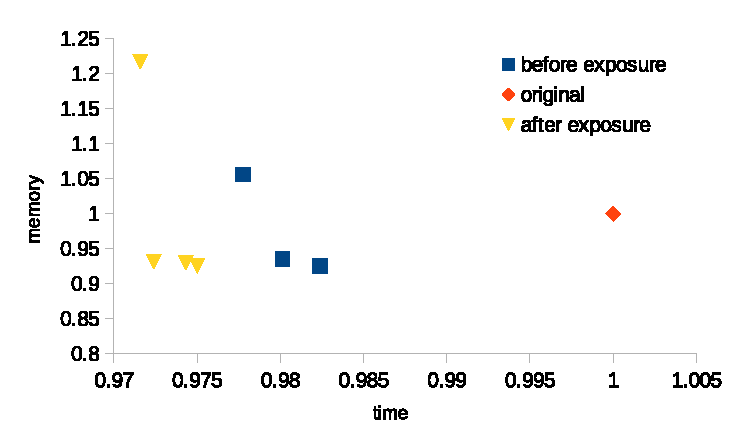
\includegraphics[width=0.4\textwidth]{fig10}
	}
	\subfigure[space]{
		\label{fig_10_2}
		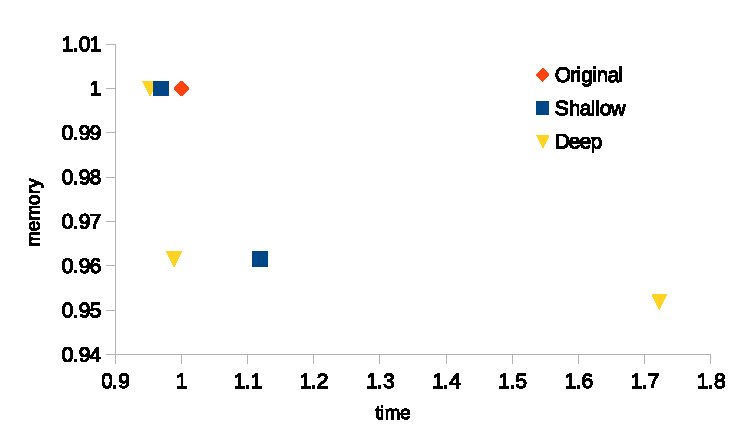
\includegraphics[width=0.4\textwidth]{fig12}
	}
	\subfigure[cfrac]{
		\label{fig_10_3}
		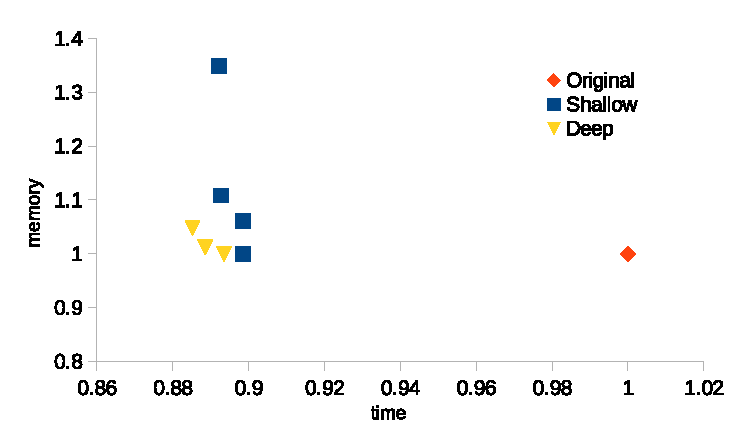
\includegraphics[width=0.4\textwidth]{fig13}
	}
	\subfigure[gawk]{
		\label{fig_10_4}
		\includegraphics[width=0.4\textwidth]{fig14}
	}
	\caption{Pareto-best individuals for each application. Less memory and time is better.}\label{fig_10}
\end{figure*}

\subsection{Shallow Parameter Tuning Improvement}

\begin{table}[hbtp]
\centering
\caption{Least memory/time consumption found by Shallow Parameter Tuning and Random Search}
\label{tab_shallow_random}
\resizebox{0.45\textwidth}{!}{
\begin{tabular}{|c|c|c|c|c|c|c|}
\hline
\multirow{2}{*}{Multi-Row} & \multicolumn{2}{|c|}{Original} & \multicolumn{2}{|c|}{Random} & \multicolumn{2}{|c|}{Shallow Parameter Tuning} \\
\cline{2-7}
& time & memory & least-time & least-memory & least-time & least-memory\\
\hline
\textbf{\emph{espresso}} & 4.82s & 5152KB & 4.70s & 4768KB & 4.73s & 4768KB \\
\hline
\textbf{\emph{space}} & 32ms & 416KB & 22ms & 404KB & 21ms & 400KB \\
\hline
\textbf{\emph{cfrac}} & 1.00s & 332KB & 0.95s & 332KB & 0.94s & 332KB \\
\hline
\textbf{\emph{gawk}} & 2.55s & 4356KB & 2.47s & 4320KB & 2.44s & 4320KB \\
\hline
\end{tabular}}
\end{table}

In order to understand whether we can improve an application by specializing \emph{dlmalloc}, and whether our search-based algorithm is effective on this problem, we first conduct Shallow Parameter Tuning on \emph{dlmalloc} and compare the results with the performance of the default and randomly generated configurations. The result is reported in Table \ref{tab_shallow_random}. 

By Shallow Parameter Tuning, we consistantly achieve better performance in terms of memory compared with the original on all applications except \emph{cfrac}. Noticing that \emph{cfrac} requires the least memory among all applications under test, it makes less difference than other applications. Compared with random search, the least-memory consumption found by Shallow Parameter Tuning is almost the same on each application, implying that the improvement is easy to be found so that improving \emph{dlmalloc} costs very little computation effort. On the time consumption, the Shallow Parameter Tuning can find better solution than both the original and random search result on all applications but \emph{espresso}. (**I'm still investigating why Shallow Parameter Tuning doesn't perform well on \emph{espresso})

This result indicates that the general-purpose allocator has the potential to be easily improved by adjusting it to a specific application. Though the multi-optimization of the shallow parameters is effective and well-guided on this problem, it cannot perform much better than the random search due to the very little computation cost to find the best. This leads us to Deep Parameter Tuning.

\subsection{Deep Parameter Tuning Improvement}

\begin{figure}[htbp]
	\centering
	\subfigure[espresso]{
		\label{fig_sig_espresso}
		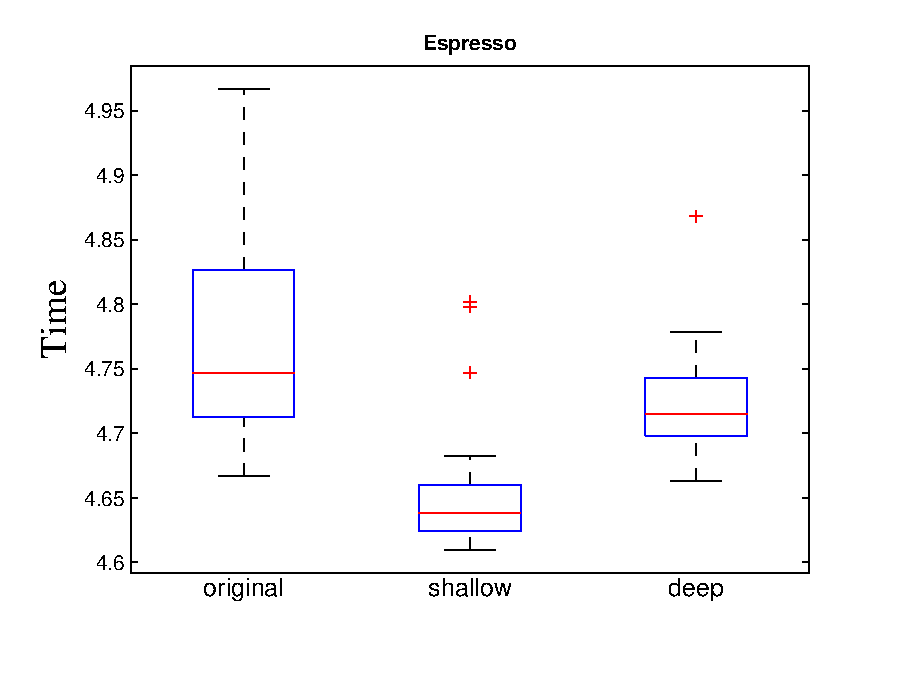
\includegraphics[width=0.2\textwidth]{espresso-small}
	}
	\subfigure[space]{
		\label{fig_sig_space}
		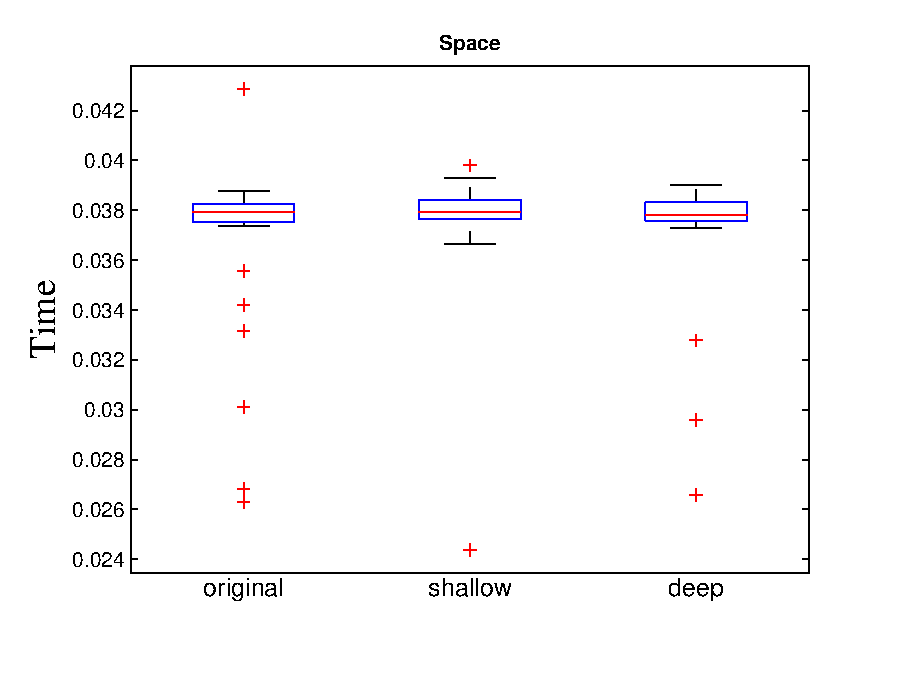
\includegraphics[width=0.2\textwidth]{space-small}
	}
	\subfigure[cfrac]{
		\label{fig_sig_cfrac}
		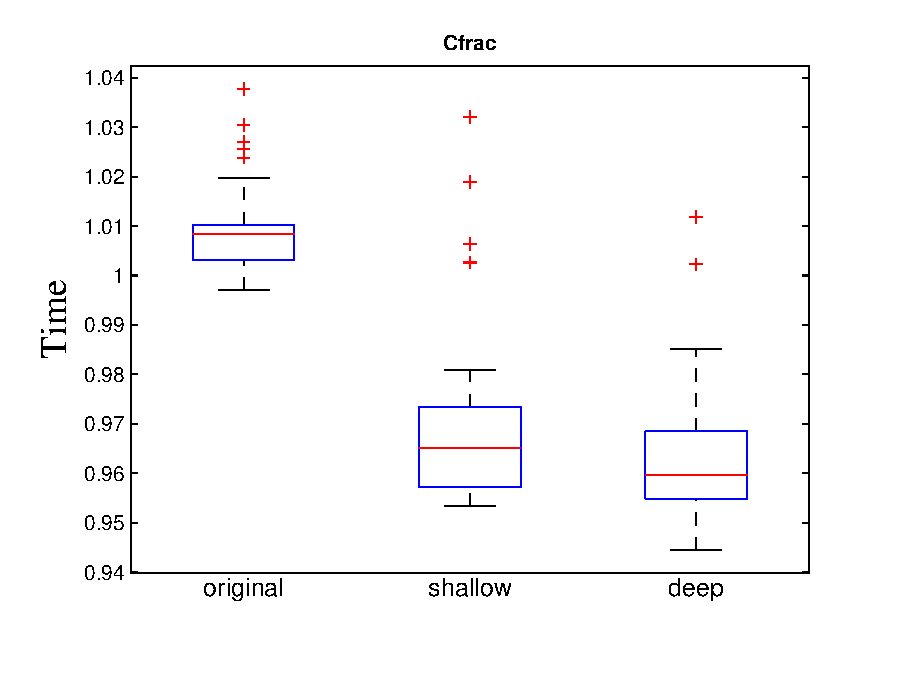
\includegraphics[width=0.2\textwidth]{cfrac-small}
	}
	\subfigure[gawk]{
		\label{fig_sig_gawk}
		\includegraphics[width=0.2\textwidth]{gawk-small}
	}
	\caption{Time consumption of the best configuration from the original, the Shallow and Deap Parameter Tuning}\label{fig_sig}
\end{figure}

Knowing the Shallow Parameter Tuning already works, but almost as well as the random search, on this optimisation problem, we want to know how much more can we achieve by the Deep Parameter Tuning. So we expose the most influential peices of code as tunable parameters and optimize them as well as the shallow parameters. 

According to the result in Figure \ref{fig_10}, we achieve up to 11\% reduction on the time consumption (gawk, Figure \ref{fig_10_4}), and 7.5\% reduction on the memory consumption (espresso, Figure \ref{fig_10_1}), compared to the default configuration. Due to the instrumentation way of memory measurement, the memory consumption is deterministic as reported. But the time consumption could fluctuate due to the system noises. In order to understand the subtle difference between the results of Shallow and Deep Parameter Tuning, the most time-saving configurations gotten from the results of these two approaches are re-test for 30 times and the time consumption is recorded. Figure \ref{fig_sig} shows that, the result from Deep Parameter Tuning is slightly better than the Shallow Parameter Tuning on \emph{cfrac} and \emph{gawk}, whilst comparable on \emph{space} and slightly worse on \emph{espresso}. From Table \ref{tab_2}, we also find that the time and memory performance can be improved at the same time. 

On the other hand, for some non-functional properties in several applications, we can't find better configuration, implying the default configuration might already be the optimal for these applications in terms of one of these properties. We also find that, the optimal configuration for one application doesn't guarantee to improve other applications, showing that the default configuration is the result of negotiation between general applications. What's more interesting is, by the Deep Parameter Tuning, we are able to find more extreme performance that widens the Pareto front. This means we could provide wider range of choices to users especially when the application has to run in an extreme environment.

\begin{table*}[hbtp]
\centering
\caption{Best individuals for each application. The square points in each graph are the non-dominated best individuals of the Deep Parameter Tuning, and the triangle points are the result of the Shallow Parameter Tuning.}
\label{tab_2}
\resizebox{0.8\textwidth}{!}{
\begin{tabular}{c|c|c|c|c}
\hline
\textbf{\emph{espresso}} & time(s) & normalized time & memory(kB) & normalized memory \\
\hline
original & 4.773 & 100\% & 5152 & 100\% \\
\hline
most-time-saving before exposure & 4.667 & 97.8\% & 5440 & 105.6\% \\
\hline
most-time-saving after exposure & 4.638 & 97.2\% & 6272 & 121.7\% \\
\hline
most-memory-saving before exposure & 4.689 & 98.2\% & 4768 & 92.5\% \\
\hline
most-memory-saving after exposure & 4.654 & 97.5\% & 4768 & 92.5\% \\
\hline
\hline
\textbf{\emph{space}} & time(ms) & normalized time & memory(kB) & normalized memory \\
\hline
original & 19.3 & 100\% & 416 & 100\% \\
\hline
most-time-saving before exposure & 18.7 & 96.9\% & 416 & 100\% \\
\hline
most-time-saving after exposure & 18.0 & 93.2\% & 416 & 100\% \\
\hline
most-memory-saving before exposure & 21.6 & 111.8\% & 400 & 96.2\% \\
\hline
most-memory-saving after exposure & 39.9 & 206.3\% & 396 & 95.2\% \\
\hline
\hline
\textbf{\emph{cfrac}} & time(s) & normalized time & memory(kB) & normalized memory \\
\hline
original & 1.071 & 100\% & 332 & 100\% \\
\hline
most-time-saving before exposure & 0.956 & 89.2\% & 448 & 134.9\% \\
\hline
most-time-saving after exposure & 0.981 & 91.6\% & 352 & 106\% \\
\hline
most-memory-saving before exposure & 0.962 & 89.8\% & 332 & 100\% \\
\hline
most-memory-saving after exposure & 1.001 & 93.5\% & 332 & 100\% \\
\hline
\hline
\textbf{\emph{gawk}} & time(s) & normalized time & memory(kB) & normalized memory \\
\hline
original & 2.711 & 100\% & 4356 & 100\% \\
\hline
most-time-saving before exposure & 2.396 & 88.4\% & 4356 & 100\% \\
\hline
most-time-saving after exposure & 2.389 & 88.1\% & 4320 & 99.2\% \\
\hline
most-memory-saving before exposure & 2.406 & 88.8\% & 4320 & 99.2\% \\
\hline
most-memory-saving after exposure & 2.389 & 88.1\% & 4320 & 99.2\% \\
\hline
\end{tabular}}
\end{table*}

(**We still need time to run the same experiments for many times, in order to show the consistency of the results)

\subsection{Understanding the Exposed Parameters}

\begin{table*}[htbp]
\centering
\caption{Exposed Parameters}
\label{tab_exposed_param}
\resizebox{\textwidth}{!}{
\begin{tabular}{|c|c|c|c|}
\hline
Line & Exposed part & Substitute options & Description \\
\hline
4059 & (use\_mmap(m) \&\& nb >= mparams.mmap\_threshold \&\& m->topsize != 0) & 2 & Enable \emph{mmap} system call\\
\hline
4144 & (m->footprint\_limit == 0 || (fp > m->footprint \&\& fp <= m->footprint\_limit)) & 4 & Predicate controling system allocation\\
\hline
4348 & TOP\_FOOT\_SIZE & numeric & Segment overhead size of the top chunk\\
\hline
4353 & ((m->topsize - pad + (unit - SIZE\_T\_ONE)) / unit - SIZE\_T\_ONE) * unit & 6 & Calculation of remaining memory when trimming\\
\hline
\end{tabular}}
\end{table*}
From the sensitivity information, we find four places that have the most impact to the performance of \emph{dlmalloc}, which are list in Table \ref{tab_exposed_param}. They locate in different functions that involve system allocation and deallocation. LINE4059 checks whether current situation meets the \emph{mmap} criteria, so it could easily enable or disable direct memory mapping. LINE4144 is also a predicate controling the extending of the heap. TOP\_FOOT\_SIZE in LINE4383 is a constant determined by some other macros and parameters. It influences how much memory should be always kept in the top chunk. LINE4353 is an expression calculating how much memory should be preserved when shrinking the heap.

After human inspection, one can easily find the exposed parameters introduced above can directly influence the memory and/or time performance of the allocator. Due to the limit space, we only elaborate one of them. TOP\_FOOT\_SIZE controls how many extra bytes should be included in the top chunk while the allocator extends the top chunk. It influences how much more memory than actually needed \emph{dlmalloc} should keep to buffer allocation and deallocation. 

Bigger TOP\_FOOT\_SIZE tends to cost more memory but possibly saves some costly system allocation and deallocation. The optimal value could vary across applications. Originally it is a constant determined by some macros and system related parameters. After made to a tunable parameter and exposed to users, it can be explicitly configured from the outside like other parameters.

To anyone who is familiar to the code, TOP\_FOOT\_SIZE as well as other exposed parameters are very obvious to have the potential to vary the performance of the allocator. So the mutation-based sensitivity analysis can not only help us discover useful internal parameters to expose, but also point them out to human developers so that the developers could pay more attention to these pieces of code and possibly improve the program with less effort.

\subsection{Threats to Validity}

Mutation-based sensitivity advantages in efficiency and automation, but it is not necessarily the best way to expose Deep Parameters in terms of the quality of the Deep Parameters. Intuitively, Mutation Operators may change a constant or an operator on an arithmatic expression, thus likely to change the value of the expression in different degrees so that we can capture the sensitivity of this expression. How good Mutation Operators are in capturing sensitivity information remains as an extension of this work.

Despite less possible, the experimental environment may differ among the virtual machines on the cloud. 

The choose of test suite could in some degree affect the results. Even with a good test suite that achieves a high branch coverage, it could still differ from the distribution of the real world inputs, in which case the optimized configuration over this testsuite may not achieve the best performance in real world situations. So the result is testsuite driven, meaning the best configuration over our testsuite is not necessarily a good one on every test case.

One other concern is whether the result holds on other applications. Despite subject applications from different fields for different uses, potential threat to our conclusion could exist beyond our test. Currently we can only claim that our approach works on the applications under test in this paper, but because of the wide range of where these applications come from, it is highly likely this approach can be easily generalized to other applications and lead to similar result on many of them.

\vspace{-2mm}

\section{Related Work}

State-of-the-art dynamic memory managers usually combine several
different allocation strategies to serve memory requests with different
sizes. Risco-Mart\'{\i}n et al.~\cite{RiscoMartín2014109,
Colmenar:2011:MOD:2001576.2001820} search for the best allocation strategy
for different sizes as well searching for the best range of sizes on which
each strategy should be applied. 
Their work requires human effort to implement the
allocation strategies. In our approach, changing the parameters not
only (indirectly) changes the separators of size ranges and allocation
strategy applied on each range, but also influences strategy behaviour. 

%Some embedded systems, especially those executing multimedia applications, suffer from massive memory usage and limited resources. Risco-Martin et al.\cite{Risco-Martin:2009:ODM:1569901.1570116}\cite{RiscoMartin2010572} decomposes memory allocators into several components, for each of which there are several optional implementations of different allocation strategies. Combining different implementations to generate the optimal dynamic memory manager (DMM) becomes a searching problem. They use grammatical evolution to solve this optimisation problem with two real world applications: Physics3D and VDrift. Other than \emph{dlmalloc}, they target the DMM on embedded systems that usually run memory-intensive applications. In their approach, they try to find the best combination of several basic strategies, different from which, we start from the state-of-the-art combination of allocation strategies and adjust its configuration to each application. 

%Grunwald and Zorn introduced \emph{CustoMalloc}, a system that customizes and synthesizes a memory allocator for a given application\cite{SPE:SPE4380230804}. The basic idea is, run an application and record all the memory allocation and deallocation during the run so that \emph{CustoMalloc} can find the most frequent sizes. Then the system generates a custom memory allocator using two allocation strategies for different sizes: fast but more overheaded way for the most frequent sizes and traditional way for other sizes. They also reported that the performance of a synthesized allocator is not sensitive to the input of the application, suggesting that for a given application, the memory allocation and deallocation patterns for different inputs are similar. In their and our works, we both try to create a custom memory allocator for each specific application but we use a simpler way, parameter tuning in one of the best allocators. Extending from that, we expose more valuable parameters from the source code and optimise them.

%Many works have studied the influence of algorithms'
%configurations or means of automatically adjusting them. For purposes of comparison
%and context, we focus on \emph{ParamILS}.
\emph{ParamILS}~\cite{hutter2009paramils} is an automatic framework proposed by Hutter et al.,
which automatically configures an algorithm's parameters to optimise
performance on a given test suite. 
% It uses a local search and computes
% fitness by running the application with each candidate configuration. 
While
targeting parameter tuning as well, our approach focuses on standard
library code, based on the assumption that the general-purpose memory
allocators may not be optimal for each specific application. In addition,
\emph{ParamILS} can only optimise existing (shallow) parameters, while our
approach exposes additional parameters and adjusts their values to gain more
improvement.

Hoffmann et al.~\cite{Hoffmann:2011:DKR:1950365.1950390} proposed
\emph{PowerDial}, a system which dynamically adjusts an application's
behaviour to make it adaptable to fluctuating workloads. 
% It first transforms
% some configuration parameters to non-constant variables residing in the
% application's memory, so the behaviour of the application can be altered by
% controlling these variables at runtime. Then it pre-runs the application
% with each possible configuration to determine how these parameters
% influence the application and memoizes the Pareto-best candidates in terms
% of application's non-functional properties and the quality of the output.
Whenever \emph{PowerDial} detects a resource shortage it sacrifices 
output quality by changing the values of variables, allowing
the application to `survive the crisis'. One limitation of
this work is that the search space of configuration variables must be small
enough to admit an exhaustive search. In our work the search space is too
large to use such an exhaustive search, and thus we applied search-based
techniques. % Similar to \emph{ParamILS}, 
\emph{PowerDial} only operates
on existing (shallow) parameters. 

Hutter et al.~\cite{4401979} have tuned the parameters of a SAT
solver, SPEAR, by adjusting not only the explicit parameters but also many
implicit parameters. They expose almost all possibly tunable variables 
and thereby a much larger search space than we do. 
% unscalable computation efforts. 
To reduce the
computation effort by limiting the search space, we use a mutation-based
technique to find the most influential parts of the code and focus the search
on just them. 
This sensitivity analysis effectively reduces the 
space, admitting practical searches.

In previous work, the Software Tuning panel for Autonomic Control 
(STAC)~\cite{Brake:2008:ADS:1370018.1370031} automated the expsoure of a
limited form of `deep' parameters. 
% STAC first generates a design graph for
% a subject under optimisation. The design graph represents data reference
% transition flows in the subject. It then uses the reference patterns of
% shallow parameters to discover deep parameters, whose reference pattern is
% the same as one of the shallow parameter reference patterns. 
Although STAC
can discover some deep parameters effectively, it suffers from two
limitations. First, STAC requires initial human effort to characterise
shallow parameters. Second, STAC can only find a subset of deep parameters,
those that have similar data transition patterns to the known shallow
parameters. To overcome these limitations, we apply a mutation-based
sensitivity analysis to fully automate the process of locating potential
deep parameters and subsequently apply NSGA-II to search for optimal values
for these parameters to balance non-functional properties of interest. 


\vspace{-2mm}
\section{Conclusions}

In this paper we propose an automatic algorithm for discovering and
optimising deep parameters to tune programs with respect to non-functional
properties.  In particular, we focus on tuning \emph{dlmalloc}, a memory
allocator, to reduce the time and memory high-water-mark requirements of
off-the-shelf programs. Our approach combines mutation analysis to
discover sensitive deep parameters as well as an SBSE approach which 
subsequently optimises these parameters, while retaining the functionality expressed in
a test suite.  In a series of experiments involving over 70,000 lines of
code and 700 test cases we found that our deep parameter approach
outperformed baseline optimisations (which use only the programmer-provided
shallow parameters), ultimately improving execution time by 12\% 
and memory consumption by 21\% in the best cases. In addition, despite
the larger search space considered, the additional optimisation time cost
of our approach is acceptably low. Overall, we feel that deep parameter tuning 
approaches show much promise for the automated improvement of software
with respect to non-functional properties.  

% FIXME: Wes Weimer found the entire conclusion below to be very hard to
% follow, so I rewrote it entirely with the text above. You should check
% that text as a starting point make sure, for example, that it does not
% contain any falsehoods.

% Fan checked the text above and it's all correct. 

\vspace{-2mm}

%\end{document}  % This is where a 'short' article might terminate

%ACKNOWLEDGMENTS are optional
\section{Acknowledgments}
**Acknowledgement. Grant.

%
% The following two commands are all you need in the
% initial runs of your .tex file to
% produce the bibliography for the citations in your paper.
\bibliographystyle{abbrv}
\bibliography{myReading}  % sigproc.bib is the name of the Bibliography in this case
% You must have a proper ".bib" file
%  and remember to run:
% latex bibtex latex latex
% to resolve all references
%
% ACM needs 'a single self-contained file'!
%
%APPENDICES are optional
%\balancecolumns

\balancecolumns
% That's all folks!
\end{document}
